\begin{frame}
	\frametitle{Recorrências}
	\begin{figure}
		\centering
		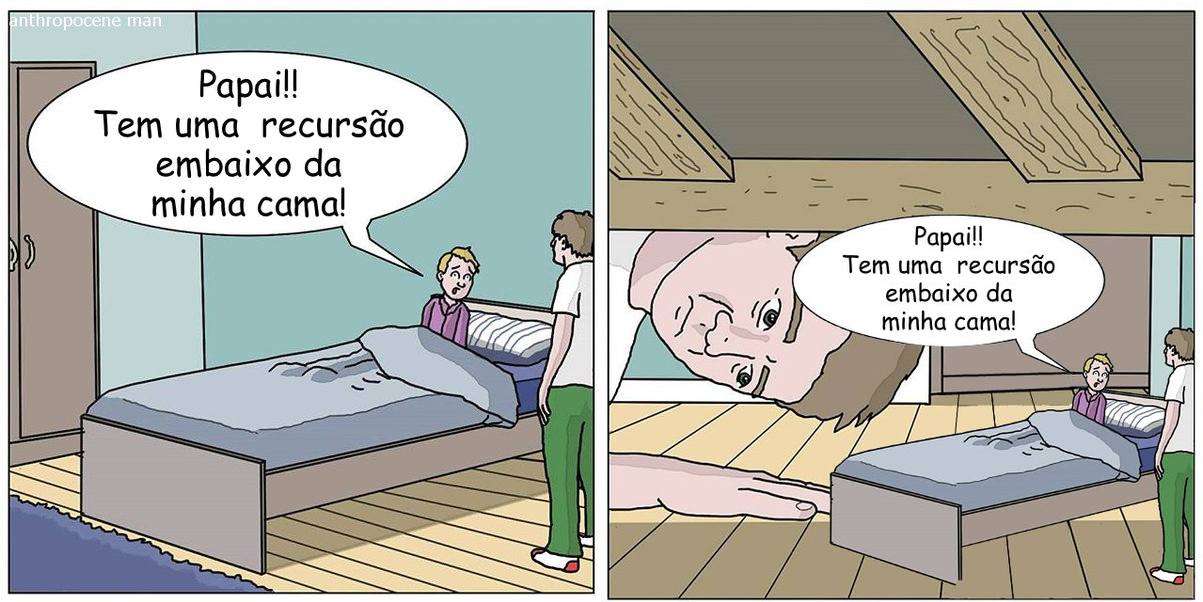
\includegraphics[width=1\linewidth]{images/recursivo}
		\caption{}
		\label{fig:recursivo}
	\end{figure}
\end{frame}

\begin{frame}
	\frametitle{Recorrências}
	\par A recorrência é uma forma de descrever o comportamento de algoritmos recursivos.\newline
	\par Para esse tipo de análise usaremos, entre outras coisas, o que se chama de \textbf{relação de recorrência}.
	\par Toda recursão tem um \textbf{caso base} ou \textbf{ponto de parada}. O caso base é o conjunto de instruções que fará com que um valor trivial seja finalmente retornado (ou não) iniciando o desempilhamento da pilha de recursão. Além disso deve existir o \textbf{caso indutivo} ou \textbf{recursão} que é o trecho de código onde a função faz uma chamada a ela mesma empilhando a chamada anterior e suas respectivas variáveis/estados.
	\lstinputlisting[language=C++]{../codigo/algoritmoRecursivo01.cpp}
\end{frame}

\begin{frame}
	\frametitle{Relações de recorrência}
	\framesubtitle{Exemplo 01}
	\par Qual a relação de recorrência desse algoritmo?\\
	\lstinputlisting[language=C++]{../codigo/algoritmoRecursivo01.cpp}
	\par Do \textbf{único} caso indutivo é possível perceber que a entrada é diminuída em \textbf{n-1}, de todo o resto do algoritmo percebe-se que os tempos de execução são constantes, ou seja, $\Theta(1)$.
	\par Então a relação de recorrência é dada por esses valores como colocado na equação \ref{eq:relRecor}. 
	\begin{equation}
		\label{eq:relRecor}
		T(n) = 1.T(n-1) + \Theta(1)
	\end{equation}
\end{frame}

\begin{frame}
	\frametitle{Relações de recorrência}
	\framesubtitle{Exemplo 02}
	\par Qual a relação de recorrência desse algoritmo?\\
	\lstinputlisting[language=C++]{../codigo/algoritmoRecursivo02.cpp}
	\par Dos \textbf{dois} casos indutivos é possível perceber que a entrada é diminuída em \textbf{n-1} e \textbf{n-2}, de todo o resto do algoritmo percebe-se que os tempos de execução são constantes, ou seja, $\Theta(1)$.
	\par Então a relação de recorrência é dada por esses valores como colocado na equação \ref{eq:relRecor01}. 
	\begin{equation}
		\label{eq:relRecor01}
		T(n) = 1.T(n-1) + 1.T(n-2) + \Theta(1)
	\end{equation}
\end{frame}


\begin{frame}
	\frametitle{Relações de recorrência}
	\framesubtitle{Exemplo 03}
	\par Qual a relação de recorrência desse algoritmo?\\
	\lstinputlisting[language=C++]{../codigo/algoritmoRecursivo03.cpp}
	\par Dos \textbf{dois} casos indutivos é possível perceber que a entrada é diminuída em \textbf{n/2} e \textbf{n-2}, de todo o resto do algoritmo percebe-se que os tempos de execução são \textbf{constantes + complexidade n}, ou seja, $\Theta(n)$.
	\par Então a relação de recorrência é dada por esses valores como colocado na equação \ref{eq:relRecor02}. 
	\begin{equation}
		\label{eq:relRecor02}
		T(n) = T(n/2) + T(n/2) + \Theta(n) + \Theta(1) \rightarrow 2.T(n/2) + \Theta(n)
	\end{equation}
\end{frame}

\begin{frame}
	\frametitle{Resolvendo relações de recorrência}
	\begin{itemize}
		\item método da árvore de recursão
		\item método iterativo
		\item método mestre
	\end{itemize}
\end{frame}

\begin{frame}
	\frametitle{Resolvendo relações de recorrência}
	\framesubtitle{Base matemática}
	\begin{columns}
		\begin{column}{0.55\textwidth}
			\begin{equation}
				\begin{aligned} 
					&\sum_{k=1}^{n} a_k = a_1 + a_2 + \dots + a_k\\
					&\sum_{k=1}^{\infty} a_k = \lim\limits_{n \to \infty} \sum_{k=1}^{n} a_k\\
					&\sum_{k=1}^{n} (c.a_k + b_k) = c.\sum_{k=1}^{n} a_k + \sum_{k=1}^{n} b_k\\
					&\sum_{k=1}^{n} \Theta(f(k)) = \Theta\left(	\sum_{k=1}^{n} f(k)\right)
				\end{aligned}
			\end{equation}
		\end{column}
		\begin{column}{0.45\textwidth}
			\begin{equation}
				\begin{aligned}
					&P.A.\\ 
					&a_n = a_1 + (n-1).r\\
					&S_n = \dfrac{n.(a_1 + a_n)}{2}\\
					&P.G.\\
					&a_n = a_1.q^{n-1}\\
					&S_n = \dfrac{a_1.(q^n-1)}{q-1} \qquad &\forall q \geq |1|\\
					&S_n = \dfrac{a_1}{1-q} \qquad &\forall q < |1|
				\end{aligned}
			\end{equation}
		\end{column}
	\end{columns}
\end{frame}

\begin{frame}
	\frametitle{Resolvendo relações de recorrência}
	\framesubtitle{Base matemática}
	\begin{columns}
		\begin{column}{0.5\textwidth}
			\begin{equation}
				\begin{aligned} 
					&\log_ca = k \Leftrightarrow c_k = a\\
					&\log_c(ab) = \log_ca+\log_cb\\
					&\log_ba^n = n.log_ba\\
					&\log_aa=1\\
					&\log n = \lg n = \log_2n\\
					&a = b^{\log_ba}\\
					&a^{\log_bn} = n^{\log_ba}\\
					&\log_ab = \dfrac{\log_cb}{\log_ca}
				\end{aligned}
			\end{equation}
		\end{column}
		\begin{column}{0.5\textwidth}
			\begin{figure}
				\centering
				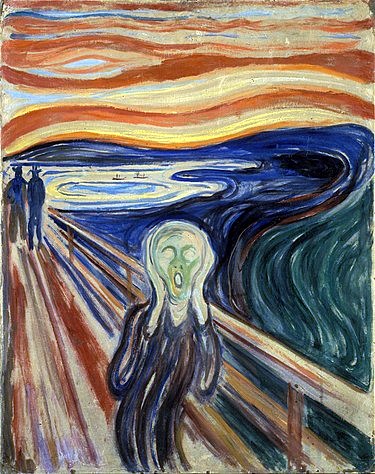
\includegraphics[width=0.7\linewidth]{images/ogrito}
				\caption{Ahhhhhhh!}
				\label{fig:ogrito}
			\end{figure}
		\end{column}
	\end{columns}
\end{frame}

\begin{frame}
	\frametitle{Resolvendo relações de recorrência - Método da árvore de recursão}
	\framesubtitle{Passos para resolver - Exemplo 0}
		\begin{columns}
		\begin{column}{0.5\textwidth}
			\begin{itemize}
				\item expandir a árvore
				\item calcular a altura \textbf{h}
			\end{itemize}
		
			\par Para entender como expandir a árvore de recursão, ao lado coloquei um exemplo simples para a seguinte relação de recorrência:
			\begin{equation}
				T(n)=T(n-1) + \Theta(1)
			\end{equation}
			\par Ao fazer a expansão se chega no caso-limite em que o tamanho da entrada é igual a 1 ($T(1)$). Dessa forma a altura $\mathbf{h=\Theta(n)}$ já que $h=n-1 \implies \Theta(n)$
		\end{column}
		\begin{column}{0.5\textwidth}
			\begin{figure}
				\centering
				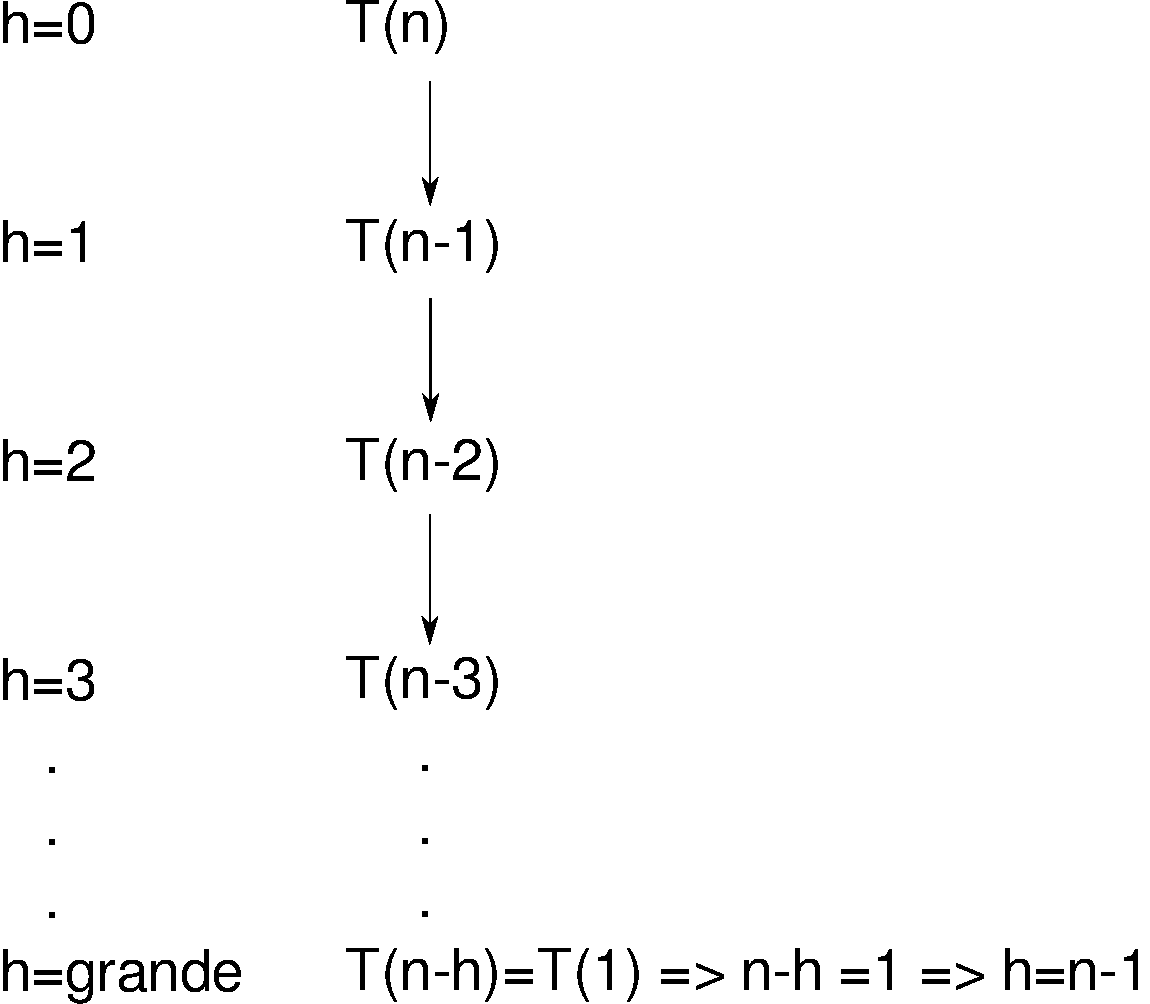
\includegraphics[width=.9\linewidth]{images/arvoreDeRecussao00}
				\caption{Árvore de recursão expandida}
				\label{fig:arvorederecussao00}
			\end{figure}
		\end{column}
	\end{columns}
\end{frame}

\begin{frame}
	\frametitle{Resolvendo relações de recorrência - Método da árvore de recursão}
	\framesubtitle{Passos para resolver - Exemplo 0}
	\begin{columns}
		\begin{column}{0.35\textwidth}
			\begin{itemize}
				\item calcular os custos por nível
				\item somatória dos custos dos níveis \textbf{h} vezes
			\end{itemize}
			\par Nesta fase devemos nos concentrar no \textbf{tempo gasto para combinar os resultados das chamadas recursivas}.\newline
			\par Esse tempo é dado pelo último termo da relação de recorrência.
		\end{column}
		\begin{column}{0.65\textwidth}
			\par Então:
			\begin{equation}
				\begin{aligned}
					&T(n) \to T(n-1) \to T(n-2) \to \dots \to T(n-h) \implies \\
					&\Theta(1) + \Theta(1) + \Theta(1) + \dots + \Theta(1)=\mathbf{\Theta(1)} \implies\\
					&h.\Theta(1) = \Theta(n).\Theta(1) = \mathbf{\Theta(n)}
				\end{aligned}
			\end{equation}
		\end{column}
	\end{columns}
\end{frame}

\begin{frame}
	\frametitle{Resolvendo relações de recorrência - Método da árvore de recursão}
	\framesubtitle{Passos para resolver - Exemplo 1}
	\begin{columns}
		\begin{column}{0.5\textwidth}
			\par Expansão da árvore ao lado.
			\begin{equation}
				T(n)=2T(n/2) + \Theta(n)
			\end{equation}
			\par Analisando a árvore de recursão nota-se que quando a profundidade da árvore atinge seu máximo a altura da mesma é expressa segundo a expressão da equação.
			\begin{equation}
				\begin{aligned}
				&T(n/2^h)=T(1) \implies \\
				&\dfrac{n}{2^h} = 1 \implies \\
				&2^h = n \implies \\
				&\mathbf{h = \log n}
				\end{aligned}
			\end{equation}
		\end{column}
		\begin{column}{0.5\textwidth}
			\begin{figure}
				\centering
				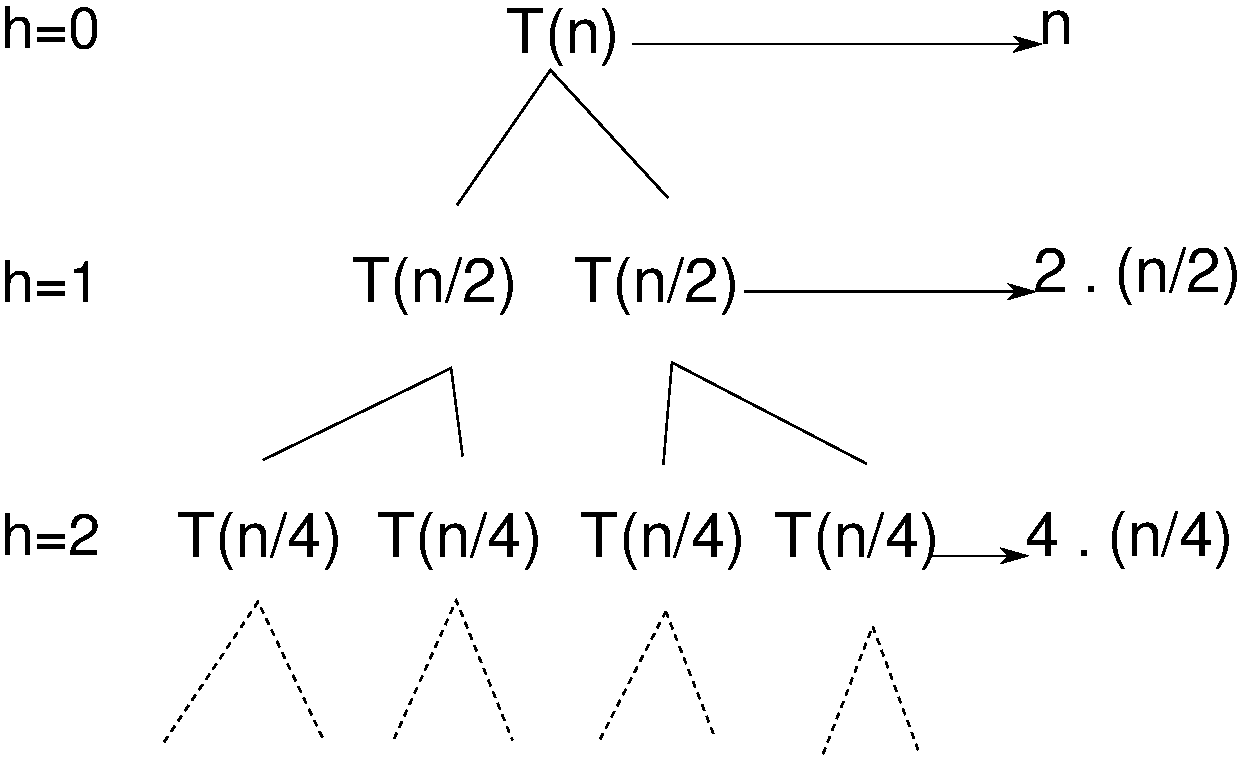
\includegraphics[width=\linewidth]{images/arvoreDeRecusao01}
				\caption{Árvore de recursão expandida}
				\label{fig:arvorederecusao01}
			\end{figure}
		\end{column}
	\end{columns}
\end{frame}


\begin{frame}
	\frametitle{Resolvendo relações de recorrência - Método da árvore de recursão}
	\framesubtitle{Passos para resolver - Exemplo 1}
	\begin{columns}
		\begin{column}{0.35\textwidth}
			\par Nesta fase devemos nos concentrar no \textbf{tempo gasto para combinar os resultados das chamadas recursivas}.\newline
			\par Esse tempo é dado pelo último termo da relação de recorrência.
		\end{column}
		\begin{column}{0.65\textwidth}
			\par Então:
			\begin{equation}
				\begin{aligned}
					&\Theta(n) + \Theta(2.n/2) + \Theta(4.n/4) + \dots + \Theta(2^h . n/2^h) = \\
					&\Theta(n)+\Theta(n)+\Theta(n)+\dots+\Theta(n) = \mathbf{\Theta(n)} \implies \\
					&h . \Theta(n) = \Theta(\log n).\Theta(n) = \mathbf{\Theta(n.\log n)}
				\end{aligned}
			\end{equation}
		\end{column}
	\end{columns}
\end{frame}

\begin{frame}
	\frametitle{Resolvendo relações de recorrência - Método da árvore de recursão}
	\framesubtitle{Exercício 0}
	\par Dadas as relações de recorrência, para cada uma, crie a árvore recursiva expandida e determine o tempo de execução do algoritmo.
	\begin{equation}
		T(n) = 3.T(n/3) + \Theta(n)
	\end{equation}
	\begin{equation}
		T(n) = 2.T(n/2) + \Theta(1)
	\end{equation}
	\begin{equation}
		T(n) = 2.T(n/3) + \Theta(1)
	\end{equation}
\end{frame}

\begin{frame}
	\frametitle{Resolvendo relações de recorrência - Método da árvore de recursão}
	\framesubtitle{Respostas}
	\begin{equation}
		T(n) = \Theta(n.\log n)
	\end{equation}
	\begin{equation}
		T(n) = \Theta(n)
	\end{equation}
	\begin{equation}
		T(n) = \Theta(n^{\log_32})
	\end{equation}
	\par No segundo e terceiros exercícios a dica é notar a progressão geométrica de \textbf{h} termos e razão 2 já que, como já foi dito, é necessário \textbf{somar h vezes} os custos.
\end{frame}

\begin{frame}
	\frametitle{Resolvendo relações de recorrência - Método da árvore de recursão}
	\framesubtitle{Exercício 1}
	\lstinputlisting[language=C++]{../codigo/algoritmoRecursivo.cpp}
	\par Qual a complexidade desse algoritmo?
\end{frame}

\begin{frame}
	\frametitle{Resolvendo relações de recorrência - Método iterativo}
	\par Dada a relação de recorrência
	\begin{equation}
		T(n) \leq T(n/2) + 1
	\end{equation}
	\par Considerando que \textbf{i} indica o número de \textbf{iterações} vamos calcular de forma \textbf{iterativa} o tempo deste algoritmo.
	\begin{equation}
		\label{eq:it1}
		T(n) \leq T(n/2) + 1 \leq T(n/2/2) + 1 + 1 \leq T(n/2/2/2) + 1 + 1 + 1 \leq \mathbf{T(n/2^i) + i} 
	\end{equation}
	\par Sendo assim, para o caso base $T(1)$, note que o tempo do algoritmo \textbf{não} depende de \textbf{i}, portanto, i é tradada como constante.
	\begin{equation}
		T(n/2^i) + i = T(1) \implies T(n/2^i) = T(1) \implies n/2^i = 1 \implies 2^i = n \implies i = \log n
	\end{equation}
	\par Substituindo \textbf{i} no resultado da equação \ref{eq:it1}.
	\begin{equation}
		T(n/2^i) + i \implies T(n/2^{\log n}) + \log n \implies T(1) + \log n \implies T(n) = \mathbf{O(\log n)}
	\end{equation}
	
\end{frame}

\begin{frame}
	\frametitle{Teorema mestre}
	\framesubtitle{Fórmula geral e limitações}
	\par É uma fórmula geral para calcular o tempo de um algoritmo mas tem algumas limitações em relação aos outros métodos já descritos:
	\begin{itemize}
		\item usado para resolver problemas do tipo "dividir para conquistar"
		\item $a =$ é o número de chamadas recursivas simultâneas
		\item $b =$ é a quantidade de subdivisões do problema
		\item $f(n)$ deve ser não negativa
	\end{itemize}
	\par Considerando essas limitações a fórmula é dada na equação \ref{eq:teorMestre}.
	\begin{equation}
		\label{eq:teorMestre}
		T(n) = a.T(n/b) + f(n)
	\end{equation}
\end{frame}

\begin{frame}
	\frametitle{Teorema mestre}
	\framesubtitle{Casos}
	\par Aplicada a fórmula, a avaliação é feita segundo as três condições abaixo:
	\begin{itemize}
		\item $f(n) = O(n^{\log_ba-\epsilon}) \exists \epsilon > 0 \implies T(n) = \Theta(n^{\log_ba})$
		\item $f(n) = \Theta(n^{\log_ba}) \implies T(n) = \Theta(n^{\log_ba}.\log_bn) = \Theta(f(n).\log_bn)$
		\item $f(n) = \Omega(n^{\log_ba+\epsilon})\exists \epsilon>0, a.f(n/b) \leq c.f(n) \forall 0 < c < 1, n=grande \implies T(n) = \Theta(f(n))$
	\end{itemize}
	\par É importante saber que o teorema mestre não necessáriamente descreve o tempo do algoritmo de forma exata: Os resultados obtidos devem ser interpretados como se referindo aos \textbf{casos médios} ou \textbf{piores casos} a depender da estrutura interna do algoritmo (instruções, desvios condicionais, etc.). Leve em consideração a possibilidade de um melhor ou pior caso que resulte em tempos excepcionais. 
\end{frame}

\begin{frame}
	\frametitle{Teorema mestre}
	\framesubtitle{Exercício}
	\par Em quais dos casos abaixo se pode aplicar o teorema mestre?
	\begin{itemize}
		\item $T(n) = 2^n.T(n/2)+n^n$
		\item $T(n) = 0,5.T(n/2)+1/n$
		\item $T(n) = 64.T(n/2) -n^2.\log n$
	\end{itemize}
	\pause
	\par Resposta: \pause \textbf{Nenhum}:
	\par Na primeiro caso o valor $2^n$ não é uma constante inteira, no segundo a mesma coisa, no terceiro $f(n)=-n^2.\log n$
\end{frame}

\begin{frame}
	\frametitle{Teorema mestre}
	\framesubtitle{Exemplo 0}
	\par Vamos resolver a relação de recorrência:
	\begin{equation}
		T(n) = 2.T(n/2) + \Theta(1)
	\end{equation}

	\begin{itemize}
		\item $a = 2$ 
		\item $b = 2$ 
		\item $f(n) = 1 = constante$ 
	\end{itemize}

	\begin{equation}
		1 < n^{\log_ba} \implies 1 < n^{\log_22} \implies 1 < n^1 \implies verdadeiro! \implies T(n)=\Theta(n^{\log_22}) = \mathbf{\Theta(n)}
	\end{equation}
\end{frame}

\begin{frame}
	\frametitle{Teorema mestre}
	\framesubtitle{Exemplo 1}
	\par Vamos resolver a relação de recorrência:
	\begin{equation}
		T(n) = 2.T(n/2) + \Theta(n)
	\end{equation}
	
	\begin{itemize}
		\item $a = 2$ 
		\item $b = 2$ 
		\item $f(n) = n$ 
	\end{itemize}
	
	\begin{equation}
		\begin{aligned}
		&n = n^{\log_ba} \implies \\
		&n = n^{\log_22} \implies \\
		&n = n^1 \implies verdadeiro! \implies \\
		&T(n)=\Theta(f(n).\log_bn) = \mathbf{n.\log n}
		\end{aligned}
	\end{equation}
\end{frame}

\begin{frame}
	\frametitle{Teorema mestre}
	\framesubtitle{Exemplo 2}
	\par Vamos resolver a relação de recorrência:
	\begin{equation}
		T(n) = 2.T(n/2) + \Theta(n^2)
	\end{equation}
	
	\begin{itemize}
		\item $a = 2$ 
		\item $b = 2$ 
		\item $f(n) = n^2$ 
	\end{itemize}
	
	\begin{equation}
		\begin{aligned}
			&n^2 > n^{\log_ba} \implies \\
			&n^2 > n^{\log_22} \implies \\
			&n^2 > n^1 \implies verdadeiro! \implies \\
			&T(n)=\Theta(f(n)) = \mathbf{\Theta(n^2)}
		\end{aligned}
	\end{equation}
\end{frame}

\begin{frame}
	\frametitle{Teorema mestre}
	\framesubtitle{Exercício 0}
	\par Vamos resolver a relação de recorrência:
	\begin{equation}
		\label{eq:tmr00}
		T(n) = 9.T(n/3) + n
	\end{equation}
	\begin{equation}
		\label{eq:tmr01}
		T(n) = 2.T(n/4)+\sqrt{n}
	\end{equation}
	\begin{equation}
		\label{eq:tmr02}
		T(n) = 3.T(n/4)+n.\log n
	\end{equation}
	
\end{frame}

\begin{frame}
	\frametitle{Teorema mestre}
	\framesubtitle{Respostas}
	\only<1>{
		\par Resolvendo a recorrência \ref{eq:tmr00}
		\par Verdadeiro para o primeiro caso:
		\begin{equation}
			\begin{aligned}
				&T(n) = 9.T(n/3) + n \implies\\
				&a=9, b=3, f(n)=n \implies\\
				&f(n) = O(n^{\log_39-\epsilon}) = \\
				&O(n^{2-\epsilon}) \implies\\
				&n \leq c.n^{2-\epsilon}, \epsilon = 1 \therefore\\
				&T(n) = \Theta(n^{\log_ba}) = \\
				&\Theta(n^{\log_39}) = \Theta(n^2)
			\end{aligned}
		\end{equation}
	}
	\only<2>{
		\par Resolvendo a recorrência \ref{eq:tmr01}
		\par Verdadeiro para o segundo caso:
		\begin{equation}
			\begin{aligned}
				&T(n) = 2.T(n/4)+\sqrt{n} \implies\\
				&a=2, b=4, f(n)=\sqrt{n} \implies\\
				&f(n) = \Theta(n^{\log_42}) \implies \\
				&\sqrt{n} = \Theta(n^{0,5}) \implies\\
				&c_1.n^{0,5} \leq \sqrt{n} \leq c_2.n^{0,5}, c_1 = c_2 = 1 \therefore\\
				&T(n) = \Theta(n^{\log_ba}.\log n) = \Theta(n^{\log_42} . \log n) =\\
				&  \Theta(n^{0,5} . \log n) =  \Theta(\sqrt{n} . \log_4 n)
			\end{aligned}
		\end{equation}
	}
	\only<3>{
		\par Resolvendo a recorrência \ref{eq:tmr02}; verdadeiro para o terceiro caso:
		\begin{equation}
			\begin{aligned}
				&T(n) = 3.T(n/4)+n.\log n \implies\\
				&a=3, b=4, f(n)=n.\log n \implies\\
				&f(n) = \Omega(n^{\log_ba + \epsilon}) \implies n.\log n = \Omega(n^{\log_43 + \epsilon}) \implies\\
				&n.\log n = \Omega(n^{0.79 + \epsilon}) \implies n.\log n = \Omega(n^{0.79 + 0,21}), \epsilon = 0,21 \implies \\
				&n.\log n = c.n^1 \implies n.\log n = \Omega(n)! \therefore\\
				&a.f(n/b) \leq c.f(n)? \implies 3.\dfrac{n}{4}.\log\left(\dfrac{n}{4}\right) \leq c.n.\log n \implies \dfrac{3n}{4}.(\log n - \log 4) \leq c.n.\log n \implies \\
				&\dfrac{3n}{4}.(\log n - 2) \leq \dfrac{3n}{4}.\log n, c=\dfrac{3}{4} \implies \log n - 2 \leq \log n \therefore T(n) = \Theta(f(n)) = \Theta(n.\log n).
			\end{aligned}
		\end{equation}
	}
\end{frame}

\begin{frame}
	\frametitle{Tudo em Todo Lugar ao Mesmo Tempo}
	\framesubtitle{Exercício}
	\par Determine a relação de recorrência do algoritmo abaixo para em seguida determinar seu tempo usando o método da \textbf{árvore de recursão}, \textbf{iterativo} e \textbf{mestre}.
	\lstinputlisting[language=C++]{../codigo/algoritmoRecursivo04.cpp}
\end{frame}